\documentclass[11pt]{report}
\usepackage[a4paper,margin=1in]{geometry}
\usepackage[T1]{fontenc}
\usepackage[utf8]{inputenc}
\usepackage{lmodern}
\usepackage{booktabs}
\usepackage{tabularx}
\usepackage{longtable}
\usepackage{array}
\usepackage{enumitem}
\usepackage{hyperref}
\usepackage{tikz}
\usetikzlibrary{arrows.meta,positioning,shapes.geometric}
\hypersetup{colorlinks=true,linkcolor=blue,urlcolor=blue}

\title{pq-signature-appliance\\Documentation Baseline}
\author{Systems Architecture Bootstrap}
\date{2026-03-16}

\begin{document}

\begin{titlepage}
  \centering
  {\Huge pq-signature-appliance\par}
  \vspace{1.2cm}
  {\Large Documentation Package\par}
  \vspace{0.8cm}
  {\large Bootstrap Baseline for ML-DSA-87 PoC on Zynq UltraScale+\par}
  \vfill
  \begin{tabular}{ll}
    Project & pq-signature-appliance \\
    Status & Bootstrap and documentation only \\
    Target Platform & Xilinx/AMD Zynq UltraScale+ \\
    External Interface & gRPC over Ethernet \\
    Internal Interface & AXI-Lite between PS and PL \\
    Signing Input & 64-byte digest \\
    Current Focus & Correctness and continuous signing \\
  \end{tabular}
  \vfill
  {\large 2026-03-16\par}
\end{titlepage}

\tableofcontents
\clearpage

\chapter{System Requirements Document}

\section*{Purpose}
This document defines the baseline requirements for the `pq-signature-appliance` proof of concept. The appliance performs ML-DSA-87 signatures on a 64-byte digest using a hardware accelerator in PL controlled by Linux software on the Zynq UltraScale+ PS.

\section{Scope}
The initial system target is a correctness-focused signing appliance with a gRPC network API and a hardware-assisted signing path. The current repository does not yet contain the actual cryptographic core implementation.

\section{Functional Requirements}
\begin{longtable}{p{0.15\textwidth} p{0.75\textwidth}}
\toprule
ID & Requirement \\
\midrule
FR-001 & The system shall expose a gRPC service for pre-hash signing requests over Ethernet. \\
FR-002 & The signing request shall contain exactly one 64-byte digest for the initial PoC API. \\
FR-003 & Linux software on the PS shall validate request shape before accessing hardware. \\
FR-004 & The PS shall communicate with the PL through an AXI-Lite wrapper interface for the PoC. \\
FR-005 & The PL-side signing path shall report busy, done, and error status to software. \\
FR-006 & The system shall return the generated signature and its reported length to the client. \\
FR-007 & The system shall support repeated signing requests during continuous operation testing. \\
FR-008 & The repository shall preserve a clean separation between software, hardware, verification, and planning artifacts. \\
FR-009 & The PoC may use hardcoded key material in PL strictly for controlled bring-up and verification. \\
FR-010 & The design shall allow later replacement of placeholder components with a real ML-DSA core without redefining the external service contract. \\
\bottomrule
\end{longtable}

\section{Non-Functional Requirements}
\begin{longtable}{p{0.15\textwidth} p{0.75\textwidth}}
\toprule
ID & Requirement \\
\midrule
NFR-001 & The initial PoC shall prioritize correctness and observability over maximum throughput. \\
NFR-002 & Architecture and interface changes shall be documented in LaTeX and planning artifacts. \\
NFR-003 & The system shall be structured for incremental multi-agent development. \\
NFR-004 & Hardware and software subsystems shall be independently testable before full integration. \\
NFR-005 & Generated EDA artifacts shall not be treated as source unless explicitly approved. \\
\bottomrule
\end{longtable}

\section{Assumptions and Exclusions}
\begin{itemize}[leftmargin=*]
  \item No third-party ML-DSA implementation is integrated at bootstrap time.
  \item Final key storage, provisioning, and production hardening are out of scope for the initial PoC.
  \item Throughput targets beyond basic modeling are deferred to later project phases.
\end{itemize}

\chapter{Preliminary Design Review}

\section*{Purpose}
This chapter captures the current architectural direction for the proof-of-concept appliance.

\section{System Objective}
The system accepts a 64-byte digest from a remote client, forwards it through a Linux-resident gRPC service, sequences a hardware signing request through AXI-Lite, and returns the resulting ML-DSA-87 signature.

\section{Top-Level Partition}
\begin{itemize}[leftmargin=*]
  \item \textbf{Client side:} submits signing requests over Ethernet.
  \item \textbf{PS software:} runs Linux, hosts the gRPC daemon, validates requests, manages MMIO, and reports status.
  \item \textbf{PL logic:} hosts the stable AXI-Lite wrapper, the ML-DSA engine adapter, project-owned ML-DSA-OSH shim logic, and the imported signing datapath.
\end{itemize}

\section{Key Architectural Choices}
\begin{itemize}[leftmargin=*]
  \item Use AXI-Lite for the initial PS and PL boundary to minimize integration complexity.
  \item Keep the external API pre-hash oriented so the service boundary is simple and deterministic.
  \item Treat continuous signing stability as a primary PoC success metric.
  \item Keep the wrapper contract independent from any single downstream ML-DSA implementation.
  \item Use an explicit engine adapter layer so ML-DSA-OSH can be attached without changing the wrapper-visible contract.
  \item Keep project-owned glue separate from the vendored third-party source tree so provenance and maintenance boundaries remain clear.
\end{itemize}

\section{Current Implementation Boundary}
The current implementation includes a real imported ML-DSA-OSH source snapshot and a real project-owned shim based on the inspected upstream sign path. The software contract and the wrapper-visible control and status surface remain unchanged. Deterministic `STUB` mode remains available for regression and bring-up.

\section{What Is Verified vs Provisional}
The wrapper contract, software path, deterministic adapter modes, and project-owned integration seam are implemented and locally verified. Full local simulation of the imported upstream sign path remains provisional because the currently available portable toolchain does not provide the mixed Verilog and VHDL elaboration flow required by the imported core.

\section{PoC Boundaries}
The proof of concept is not intended to be the final production architecture. The current design accepts higher software overhead, a temporary PoC key-provisioning model, and partial local verification limits in exchange for easier bring-up and a stable interface that future optimized implementations can preserve.

\section{Deferred Topics}
Deferred topics include production key management, end-to-end target-board validation, peak throughput optimization, secure boot interactions, and packaging for field deployment.
\chapter{Interface Control Document}

\section*{Purpose}
This chapter defines the baseline interface contracts between the external client and the appliance, and between PS software and PL logic.

\section{External Service Interface}
The appliance exposes a gRPC service named `SigningService` with a `SignPrehash` method. The request contains a single digest field that shall be exactly 64 bytes. The response returns signature bytes, a reported signature length, and a coarse status string for the PoC.

\section{External Interface Semantics}
\begin{itemize}[leftmargin=*]
  \item Requests that do not contain exactly 64 digest bytes shall be rejected in software.
  \item The PoC service processes one signing operation at a time unless future software updates explicitly add queueing.
  \item The service shall surface hardware timeout or error conditions to the client.
\end{itemize}

\section{PS/PL Interface}
The PS/PL boundary is an AXI-Lite register interface. Software writes command and digest registers, triggers execution, polls or waits for completion, and reads status plus signature output data.

\section{Interface Stability Rules}
\begin{itemize}[leftmargin=*]
  \item Changes to the gRPC message contract require matching updates to proto files and software architecture documentation.
  \item Changes to register-level behavior require matching updates to the wrapper specification and register map.
  \item Future core integration must preserve the PS-visible control semantics unless explicitly reviewed.
\end{itemize}

\chapter{ML-DSA AXI Wrapper Specification}

\section*{Purpose}
This chapter specifies the stable PoC AXI-Lite wrapper that presents the hardware signing engine to Linux software.

\section{Design Intent}
The wrapper provides a narrow, deterministic control and status surface between PS software and PL logic. It remains intentionally simple so that software, simulation, and future core refinement can converge on a stable contract.

\section{Current Implemented Structure}
The repository contains a stable AXI-Lite wrapper that instantiates a generic ML-DSA engine adapter. The wrapper owns the PS-visible register map and sequencing contract, while the adapter and downstream shim own engine-facing completion behavior.

\section{Primary Functions}
\begin{itemize}[leftmargin=*]
  \item Accept a 64-byte digest written by software.
  \item Expose control bits for start and clear-status behavior.
  \item Report idle, busy, done, and error status.
  \item Expose signature length and a read window for signature data.
  \item Remain agnostic to whether the adapter is operating in `STUB`, `CORE\_PLACEHOLDER`, or `MLDSA\_OSH` mode.
\end{itemize}

\section{Wrapper-to-Adapter Boundary}
The wrapper launches the adapter with a `start` event and a 64-byte digest, then waits for adapter completion. The adapter returns busy, done, error, signature length, and signature buffer information. The wrapper does not encode knowledge of ML-DSA-OSH internal state machines, stream ordering, or key segmentation.

\section{Current Behavioral Model}
The wrapper operates as a single-request engine for the current phase. Software shall not issue a new `start` command while the wrapper reports busy. A valid `start` clears stale visible results, launches the adapter, and later exposes a mode-dependent result once the adapter reports completion or error.

\section{Current Adapter Modes}
\begin{itemize}[leftmargin=*]
  \item \textbf{STUB:} fixed 128-byte signature, deterministic two-cycle completion latency, and signature content `STUBSIG || digest || zero padding`.
  \item \textbf{CORE\_PLACEHOLDER:} fixed 128-byte signature, deterministic four-cycle completion latency, and placeholder content `COREPH || digest || zero padding`.
  \item \textbf{MLDSA\_OSH:} real imported-core attachment path behind the adapter. When the real mixed-language core is available, the wrapper reports the actual ML-DSA-87 signature length. In the current local Verilog-only regression flow, this mode is tested through an honest fallback that reports engine error instead of claiming cryptographic success.
\end{itemize}

\section{Control Semantics}
\begin{itemize}[leftmargin=*]
  \item `start`: launches a new adapter transaction when the wrapper is not busy.
  \item `clear\_status`: clears done and error state, and clears the exposed signature buffer when the wrapper is idle.
\end{itemize}

\section{Error Handling}
The wrapper reports an error if software attempts to start a new transaction while busy or touches an unsupported register region. It also reports an engine error when the downstream adapter signals failure, including the current local `MLDSA\_OSH` fallback case used when the real imported core is not elaborated.

\section{Compatibility Note}
The register base offsets are unchanged from earlier phases. The signature-data window has been compatibly extended so the wrapper can surface the larger real ML-DSA-87 signature without introducing a new register-bank concept or changing software-visible control semantics.
\chapter{Hardware Microarchitecture}

\section*{Purpose}
This chapter describes the current PL-side organization at a level suitable for integration planning and early verification.

\section{Current Block Structure}
\begin{itemize}[leftmargin=*]
  \item \textbf{AXI-Lite wrapper:} register decode, digest staging, command acceptance, status reporting, and signature readback windows.
  \item \textbf{ML-DSA engine adapter:} stable internal boundary that accepts wrapper-level start and digest inputs and returns busy, done, error, signature length, and signature data.
  \item \textbf{ML-DSA-OSH shim:} project-owned stream adapter that formats the appliance digest input, partitions PoC key material, sequences the imported sign transaction, and reorders signature output for the wrapper-visible buffer.
  \item \textbf{Imported ML-DSA-OSH core path:} vendored third-party sign implementation under `hw/ip/mldsa\_osh/upstream/`.
  \item \textbf{Signature buffer exposure:} wrapper-visible byte window populated from adapter output once an operation completes.
\end{itemize}

\section{Current Adapter Modes}
The adapter supports three modes:
\begin{itemize}[leftmargin=*]
  \item \textbf{STUB mode:} deterministic fake-signature behavior used to validate wrapper sequencing and software integration.
  \item \textbf{CORE\_PLACEHOLDER mode:} deterministic seam-testing mode that preserves the same adapter contract while standing in for downstream core attachment.
  \item \textbf{MLDSA\_OSH mode:} real attachment path that instantiates project-owned shim logic for the imported ML-DSA-OSH sign interface.
\end{itemize}

\section{Clocking and Reset}
The initial implementation assumes a single primary PL clock domain for the wrapper and adapter path. Reset behavior forces the wrapper into an idle, non-busy state with cleared status and an empty signature window. The ML-DSA-OSH shim additionally applies a short internal reset sequence before launching the upstream sign operation.

\section{Current Dataflow}
Software writes the digest into wrapper-visible registers and asserts `start`. The wrapper launches the adapter. In `STUB` and `CORE\_PLACEHOLDER` modes, the adapter returns a deterministic local result. In `MLDSA\_OSH` mode, the shim converts the digest-oriented appliance request into the inspected upstream sign stream, captures the real core output stream, and reorders it into the wrapper-visible signature buffer.

\section{Digest Adaptation}
The appliance boundary remains digest-oriented, while the inspected upstream sign path expects formatted message bytes. The current shim therefore uses a provisional PoC adaptation that emits `0x00 || 0x00 || digest[63:0]` as the formatted message payload and provides `mlen = 64`. This assumption is isolated inside project-owned shim logic and documented explicitly so it can be revisited later without changing the wrapper or software interface.

\section{Signature Buffering}
The deterministic modes still report 128-byte signatures. The real ML-DSA-87 path uses a 4627-byte signature. To keep the wrapper contract stable while supporting the real path, the `SIG\_DATA` window has been compatibly sized for the largest supported result. The `SIG\_LENGTH` register continues to report the actual valid byte count for the selected engine mode.

\section{Adapter Rationale}
The adapter prevents the AXI-Lite wrapper from depending directly on ML-DSA-OSH-specific handshake, key-segment ordering, or output-stream ordering details. This allows the PS-visible contract to remain stable while the downstream engine implementation evolves from deterministic scaffolding to a real hardware core.

\section{Current Verification Constraint}
The imported ML-DSA-OSH sign path mixes Verilog and VHDL sources. The current local portable toolchain is sufficient for wrapper-level regression and for honest testing of the ML-DSA-OSH fallback behavior, but not for full local simulation of the mixed-language imported sign path. That limitation is tooling-related rather than an architectural decision.
\chapter{Software Architecture}

\section*{Purpose}
This chapter defines the current Linux-side software structure hosted on the Zynq PS.

\section{Current Implemented Structure}
The repository contains both a deterministic local development path and a target-facing real-MMIO bring-up path. The public software contract remains unchanged: the daemon accepts a 64-byte digest, sequences the MMIO device abstraction, and returns signature bytes plus status.

\section{Current Components}
\begin{itemize}[leftmargin=*]
  \item \textbf{Service core:} transport-independent signing orchestration over the device abstraction.
  \item \textbf{MMIO device abstraction:} stable software API for digest writes, start, wait, readback, and clear-status behavior.
  \item \textbf{Fake backend:} deterministic local register model used for unit tests, local self-test, and client smoke checks.
  \item \textbf{Real backend:} PoC user-space MMIO backend intended for Linux on Zynq, using a `/dev/mem`-style mapping path and the documented wrapper base address.
  \item \textbf{Probe helper:} safe register-visibility path that does not trigger signing.
  \item \textbf{STUB selftest path:} explicit one-transaction bring-up path that validates the deterministic STUB signature rule.
\end{itemize}

\section{Backend Selection}
Backend selection is configuration-driven. The default remains `fake`, so local development continues to work exactly as before. The `real` backend is selected through environment variables or command-line overrides and requires platform-specific MMIO mapping inputs such as the wrapper base address.

\section{Current Bring-Up Role}
The software stack is now prepared for the first real board interaction in STUB mode. The real probe command checks register visibility, and the real selftest writes a known digest, starts one operation, waits for completion, reads the signature, and compares it against the documented deterministic STUB rule.

\section{Current Claim Boundary}
The repository now contains the software infrastructure required for first PS-to-PL bring-up in STUB mode, but it does not yet claim that target-board register access or STUB selftest has been validated on actual hardware.
\chapter{Verification and Validation Plan}

\section*{Purpose}
This chapter defines the current verification strategy for the appliance.

\section{Current Verification Goal}
The current phase validates that the external request path, MMIO sequencing, wrapper behavior, imported-core integration seam, and STUB-mode board-bring-up infrastructure are stable enough to support first execution on actual Zynq hardware.

\section{Verification Layers}
\begin{longtable}{p{0.22\textwidth} p{0.68\textwidth}}
\toprule
Layer & Objective \\
\midrule
Documentation review & Confirm consistency across requirements, architecture, interfaces, planning, prompts, and STUB-mode bring-up guidance. \\
Software unit tests & Validate request checking, fake backend behavior, backend selection, probe logic, real-backend file-mapping sanity, and STUB selftest behavior. \\
Wrapper and adapter testbench & Validate reset, digest writes, start-to-busy transition, deterministic completion, signature readback, and all currently supported wrapper-visible engine modes. \\
Imported-core inspection & Confirm that project-owned shim logic is based on the actual imported ML-DSA-OSH sign path rather than assumptions. \\
STUB-mode board bring-up & Prepare safe register-visibility and one-transaction STUB validation on the actual target board. \\
\bottomrule
\end{longtable}

\section{Acceptance Focus for the Current Phase}
The current phase is accepted on interface stability, reproducible STUB-mode bring-up preparation, practical board-facing scripts, and preservation of the local development flow. It is explicitly not accepted on the basis of already-proven execution on real hardware.

\section{Current Test Assets}
\begin{itemize}[leftmargin=*]
  \item Python unit tests for digest validation and fake backend state transitions
  \item Python contract tests for the local client and service path
  \item Python tests for backend selection, probe behavior, file-backed real-backend sanity, and STUB selftest behavior
  \item A SystemVerilog wrapper testbench that covers `STUB`, `CORE\_PLACEHOLDER`, and the documented `MLDSA\_OSH` fallback behavior
  \item Imported-core inspection notes tied to the actual upstream source files
\end{itemize}

\section{Current Limits}
The imported upstream sign path still requires stronger mixed-language validation than the local portable toolchain currently provides. In addition, STUB-mode board validation still depends on actual Zynq hardware, a real AXI base address, and Linux MMIO permissions.

\section{Key Exit Criteria}
\begin{itemize}[leftmargin=*]
  \item Deterministic `STUB` mode remains simulation-backed for regression.
  \item The software stack can perform a real-backend register probe without API churn.
  \item The real selftest path checks the documented STUB signature rule explicitly.
  \item The repository is ready for a follow-on phase that performs actual STUB-mode board execution.
\end{itemize}
\chapter{Basic Performance Model}

\section*{Purpose}
This chapter provides a first-order latency model for the PoC signing path.

\section{Latency Decomposition}
The end-to-end signing latency may be approximated as:
\[
T_{total} = T_{grpc} + T_{validation} + T_{mmio\_setup} + T_{sign} + T_{mmio\_readback} + T_{response}
\]
where $T_{sign}$ is expected to dominate once the real hardware core is integrated.

\section{PoC Interpretation}
For the initial design, the control path is intentionally simple. This increases software overhead but reduces integration risk and improves observability during bring-up.

\section{Expected Bottlenecks}
\begin{itemize}[leftmargin=*]
  \item AXI-Lite register programming overhead
  \item Synchronous service behavior during the PoC
  \item Signature readback volume relative to simple control transactions
\end{itemize}

\section{Modeling Use}
This model is intended to guide architectural decisions and instrumentation points, not to claim final platform performance.

\chapter{Detailed Throughput Model}

\section*{Purpose}
This chapter extends the basic latency model into a throughput-oriented view while keeping the PoC focus on correctness.

\section{Single-Engine Throughput Approximation}
For a single in-flight engine, approximate throughput is:
\[
Throughput \approx \frac{1}{T_{mmio\_setup} + T_{sign} + T_{mmio\_readback} + T_{software\_overhead}}
\]

\section{Dominant Terms}
\begin{itemize}[leftmargin=*]
  \item $T_{sign}$ will depend on the eventual ML-DSA hardware implementation.
  \item $T_{mmio\_readback}$ scales with signature transfer volume and wrapper organization.
  \item $T_{software\_overhead}$ includes daemon scheduling, validation, and response handling.
\end{itemize}

\section{PoC Scenarios}
\begin{longtable}{p{0.22\textwidth} p{0.68\textwidth}}
\toprule
Scenario & Interpretation \\
\midrule
Conservative & Single request at a time, explicit polling, and maximal logging for bring-up. \\
Nominal PoC & Single request at a time with stable register access and reduced debug noise. \\
Future optimized & Improved transport, buffering, or hardware interface beyond AXI-Lite if required. \\
\bottomrule
\end{longtable}

\section{Guidance}
The project should instrument these latency components early so later optimization decisions are based on measured data rather than assumptions.

\chapter{Detailed Register Map}

\section*{Purpose}
This chapter defines the stabilized AXI-Lite register map implemented by the software fake backend and the RTL wrapper.

\section{Register Summary}
\begin{longtable}{p{0.14\textwidth} p{0.19\textwidth} p{0.12\textwidth} p{0.45\textwidth}}
\toprule
Offset & Name & Access & Description \\
\midrule
0x000 & CONTROL & RW & Start and clear-status control bits. \\
0x004 & STATUS & RO & Idle, busy, done, and error status indicators. \\
0x008 & ERROR\_CODE & RO & Coarse error code for wrapper or engine-detected failure. \\
0x00C & SIG\_LENGTH & RO & Reported signature length in bytes. \\
0x010-0x04C & DIGEST[0:15] & RW & Sixteen 32-bit words holding the 64-byte input digest. \\
0x100-0x1310 & SIG\_DATA[0:1156] & RO & Signature read window sized for the largest supported mode result. Deterministic modes use the leading 128 bytes; ML-DSA-87 uses up to 4627 bytes. \\
\bottomrule
\end{longtable}

\section{Control Register Bits}
\begin{itemize}[leftmargin=*]
  \item Bit 0: `start`
  \item Bit 1: `clear\_status`
\end{itemize}

\section{Status Register Bits}
\begin{itemize}[leftmargin=*]
  \item Bit 0: `idle`
  \item Bit 1: `busy`
  \item Bit 2: `done`
  \item Bit 3: `error`
\end{itemize}

\section{Current Wrapper Semantics}
\begin{itemize}[leftmargin=*]
  \item Software shall fully populate the digest registers before asserting `start`.
  \item `start` shall transition the wrapper to busy when idle.
  \item The adapter completes after a mode-specific delay or reports an engine error.
  \item `clear\_status` clears done and error latches and clears the signature window when the wrapper is idle.
  \item `SIG\_LENGTH` reports the valid byte count for the selected engine mode.
\end{itemize}

\section{Current Engine-Mode Semantics}
\begin{itemize}[leftmargin=*]
  \item `STUB`: `STUBSIG || digest || zero padding`, fixed length 128 bytes, deterministic two-cycle completion.
  \item `CORE\_PLACEHOLDER`: `COREPH || digest || zero padding`, fixed length 128 bytes, deterministic four-cycle completion.
  \item `MLDSA\_OSH`: real imported-core attachment path. The intended success case reports the real ML-DSA-87 signature length of 4627 bytes. In the current local Verilog-only regression flow, this mode is exercised via a documented fallback that reports engine error and zero signature length instead of claiming success.
\end{itemize}

\section{Current Error Codes}
\begin{itemize}[leftmargin=*]
  \item 0: no error
  \item 1: start requested while busy
  \item 2: unsupported register offset touched by the current wrapper implementation
  \item 3: engine adapter error, including the current local `MLDSA\_OSH` fallback path when the real core is not elaborated
\end{itemize}

\section{Compatibility Note}
The register base offsets are unchanged from earlier phases. The only compatible extension in the current phase is the larger readable extent of the `SIG\_DATA` window so the wrapper can expose the full ML-DSA-87 result without changing the logical register-bank structure.
\chapter{System Block Diagram}

\begin{figure}[h]
\centering
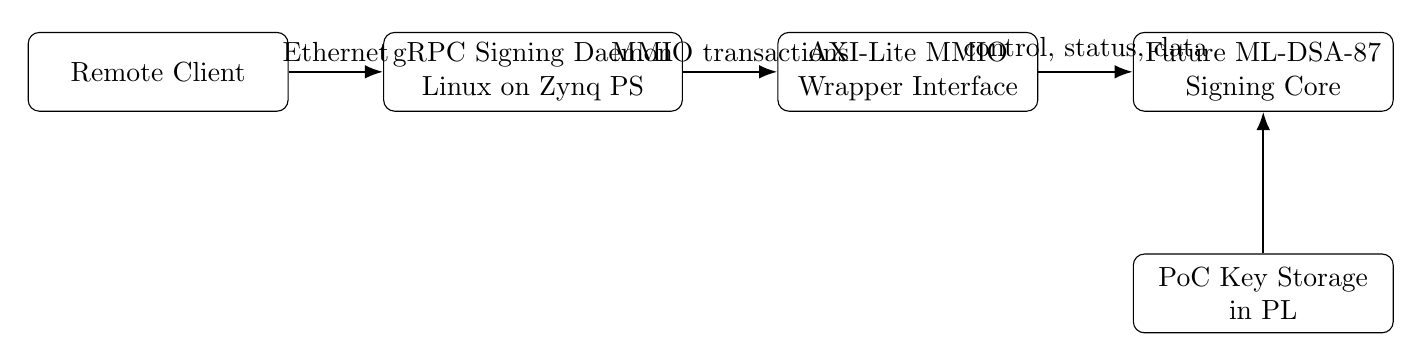
\begin{tikzpicture}[
  node distance=1.8cm and 1.2cm,
  block/.style={draw, rounded corners, minimum width=3.3cm, minimum height=1cm, align=center},
  line/.style={-Latex, thick}
]
\node[block] (client) {Remote Client};
\node[block, right=of client] (grpc) {gRPC Signing Daemon\\Linux on Zynq PS};
\node[block, right=of grpc] (axi) {AXI-Lite MMIO\\Wrapper Interface};
\node[block, right=of axi] (core) {Future ML-DSA-87\\Signing Core};
\node[block, below=of core] (keys) {PoC Key Storage\\in PL};

\draw[line] (client) -- node[above] {Ethernet} (grpc);
\draw[line] (grpc) -- node[above] {MMIO transactions} (axi);
\draw[line] (axi) -- node[above] {control, status, data} (core);
\draw[line] (keys) -- (core);
\end{tikzpicture}
\caption{Initial proof-of-concept system partition.}
\end{figure}

The diagram emphasizes the intended separation between the network service, PS-side orchestration, wrapper boundary, and PL-resident signing function.

\chapter{ML-DSA Datapath Diagram}

\begin{figure}[h]
\centering
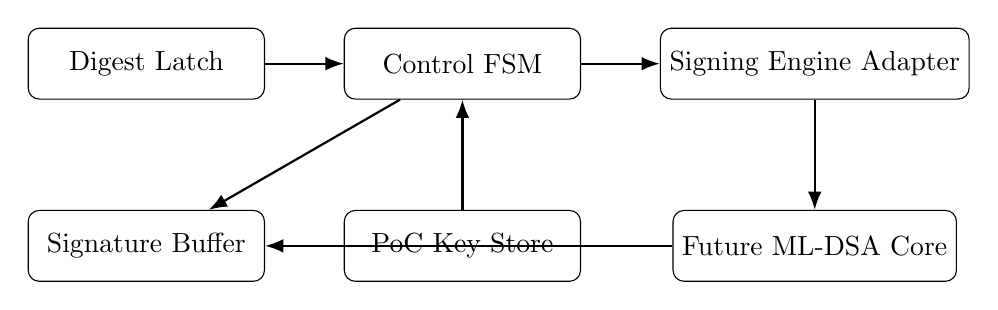
\begin{tikzpicture}[
  node distance=1.4cm and 1.0cm,
  block/.style={draw, rounded corners, minimum width=3cm, minimum height=0.9cm, align=center},
  line/.style={-Latex, thick}
]
\node[block] (digest) {Digest Latch};
\node[block, right=of digest] (ctrl) {Control FSM};
\node[block, right=of ctrl] (adapter) {Signing Engine Adapter};
\node[block, below=of adapter] (engine) {Future ML-DSA Core};
\node[block, below=of ctrl] (keys) {PoC Key Store};
\node[block, left=of keys] (sigbuf) {Signature Buffer};

\draw[line] (digest) -- (ctrl);
\draw[line] (ctrl) -- (adapter);
\draw[line] (adapter) -- (engine);
\draw[line] (keys) -- (ctrl);
\draw[line] (engine) -- (sigbuf);
\draw[line] (ctrl) -- (sigbuf);
\end{tikzpicture}
\caption{Abstract PL-side datapath organization used for planning and wrapper integration.}
\end{figure}

This diagram is intentionally abstract. It defines integration boundaries and responsibilities without committing to a concrete cryptographic microarchitecture.


\end{document}
